\chapter{Developement of a control strategy}

With a dynamic representation of the robot implemented in Matlab, control strategies can be developed and implemented. 
Two types of model-based control that are of interest for serial link manipulators were picked.

\section{Computed torque Control}
With computed torque control, the current position and velocity of the manipulator are measured. Then all non-linearities are cancelled so that only the torque needed to overcome the inertia of the actuator needs to be applied as seen in equation \ref{eq:Torquecontr_noPD}. (\cite{MathIntroRobManip} sec.5.2, P.190)
\textit{It belongs to a class of controllers known as inverse dynamic control. The principle is that the non-linear system is cascaded with its inverse so that the overall system has a constant unity gain.} \cite{CorkeRoboticVisionControl}, sect. 9.4.2, p.274\\
\begin{equation}\label{eq:Torquecontr_noPD}
	\Upsilon = M(\theta)\ddot{\theta}_d + C(\theta,\dot{\theta})\dot{\theta} + N(\theta,\dot{\theta})
\end{equation}
To correct for the difference between initial position and velocity of the manipulator and its desired states, state feedback can be added as seen in equation \ref{eq:Torquecontr}.The position error is $e=\theta - \theta_d $ and $\dot{e}$ is calculated similar. $K_v$ and $K_p$ are the position and velocity gain matrices. \cite{MathIntroRobManip}
\begin{equation}\label{eq:Torquecontr}
	\Upsilon = M(\theta)(\ddot{\theta}_d -K_v \dot{e} - K_p e) + C(\theta,\dot{\theta})\dot{\theta} + N(\theta,\dot{\theta})
\end{equation}

\section{Workspace control}
Instead of controlling the end-effector in joint space, a control in the Cartesian operational space is also possible. 
With this control scheme, the computationally intensive inverse kinematic problem does not need to be solved at each instant in time to generate a desired joint angle trajectory path. Also the feedback gains can be chosen for the directions in Cartesian space rather than for the individual joints. Trajectories in response to inputs follow a straight line in Cartesian space rather than in joint space. (\cite{MathIntroRobManip} sec.5.4, P.195)\\
\\
With the Jacobian given in \fullref{sec:Jacobian}, the dynamics can be mapped into Cartesian space by exchanging joint space coordinates for cartesian coordinates as seen in equation \ref{eq:DyanmicsMapped}. After substituting suitable expressions, and pre-multiplying by $ J^{-T} = (J^{-1})^{-T}$, following equation can be obtained:\\
\begin{equation} \label{eq:DyanmicsMapped}
	J^{-T} M(\theta) J^{-q} \ddot{x} + (J^{-T} C(\theta,\dot{\theta}) J^{-1} +J^{-T} M(\theta) \frac{d}{dt} (J^{-1}))\dot{x} + J^{-T} N(\theta, \dot{\theta}) = J^{-T}  \Upsilon
\end{equation}
By redefining the dynamics matrices as\\
$ \tilde{M} = J^{-T} M J^{-1}$\\
$ \tilde{C} = J^{-T} (C J^{-1} + M \frac{d}{dt} (J^{-1}))$\\
$ \tilde{N} = J^{-T} N$\\
$ F = J^{-T} \Upsilon$\\
The dynamics become\\

\begin{equation}
	\tilde{M} (\theta) \ddot{x} + \tilde{C} (\theta, \dot{\theta}) \dot{x} + \tilde{N} (\theta,\dot{\theta}) = F
\end{equation}

This allows to extend the computed torque control to workspace coordinates as seen in equation \ref{eq:workspaceContrFromCompTorqueContr}. $x_d$ is the desired workspace trajectory and $ e=x-x_d$ is the workspace error. 
\begin{equation} \label{eq:workspaceContrFromCompTorqueContr}
	F=\tilde{M} (\theta) (\ddot{x_d} - K_v \dot{e} - K_p e ) + \tilde{C}(\theta,\dot{\theta})\dot{x} + \tilde{N}(\theta,\dot{\theta})
\end{equation}
As the motors are still controlled in joint space, the torques can be found with \\
$\Upsilon = J^T F$\\


\section{Implementation}

These control schemes can be implemented in Simulink.  

\subsection{Computed Torque Control}
In figure \ref{fig:CompTorqueContr} the computed torque control together with a Simulink representation of the robot can be seen. 
The gains $Kp$ and $Kd$ have been determined by trial and error. 
The desired path is fed into the controller together with the states of the robot. The controller calculates the Torque and sends it to the robot.


\begin{figure}[H]
	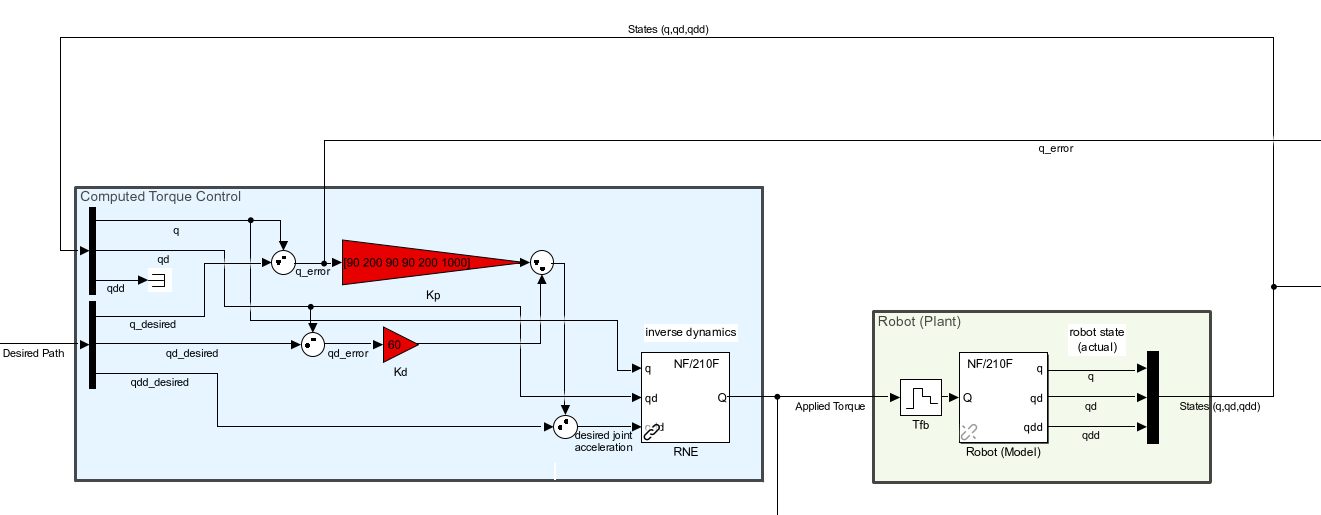
\includegraphics[
	width=1\linewidth,
	center,
	keepaspectratio,
	]{controlScheme/ComputedTorqueControl_Simulink}
	\caption{Simulink implementation of the computed Torque Control in Simulink}
	\label{fig:CompTorqueContr}
\end{figure}



\subsection{Workspace Control}
In figure \ref{fig:WorkSpaceContr} the workspace control with a Simulink representation of the robot can be seen.
The gains $Kp$ and $Kv$ have been determined by trial and error.
The desired path is fed into the controller as a transformation matrix as well as in $[X,Y,Z,Roll,Pitch,Yaw]$ coordinates.
For calculating the workspace error, a toolbox function is used. As this function has a bug, the $X$ and $Roll$ error need to be multiplied by $-1$.

\begin{figure}[H]
	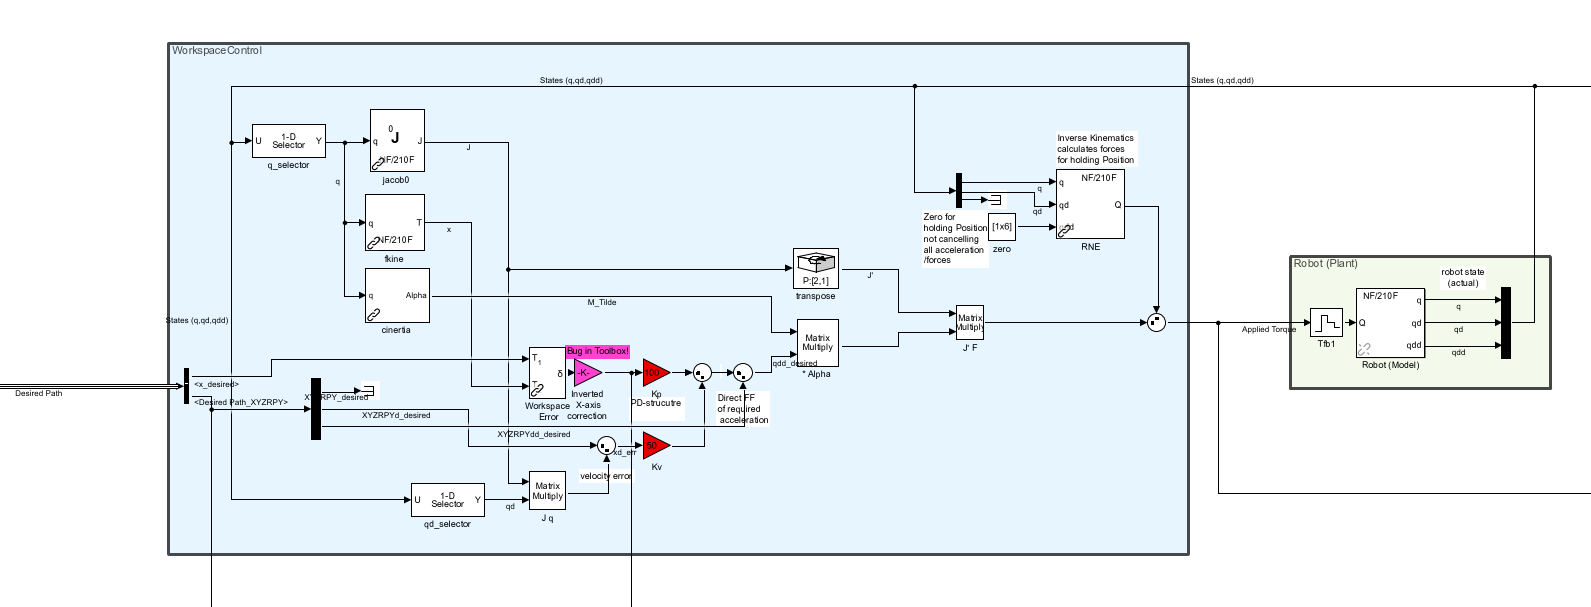
\includegraphics[
	width=1\linewidth,
	center,
	keepaspectratio,
	]{controlScheme/WorkspaceControl_Simulink}
	\caption{Workspace Control in Simulink}
	\label{fig:WorkSpaceContr}
\end{figure}


\subsection{Path Generation}
The input path to follow is generated by adjustable constants and function generators for circles, sine and others. 
The set values are close to normal pose with an offset of $1m$ in $Z$.
These individual manipulations in all six \ac{DOF} need to be fused together into a transformation matrix. 
Additionally, the desired velocity and acceleration are calculated for better accuracy. 

\begin{figure}[H]
	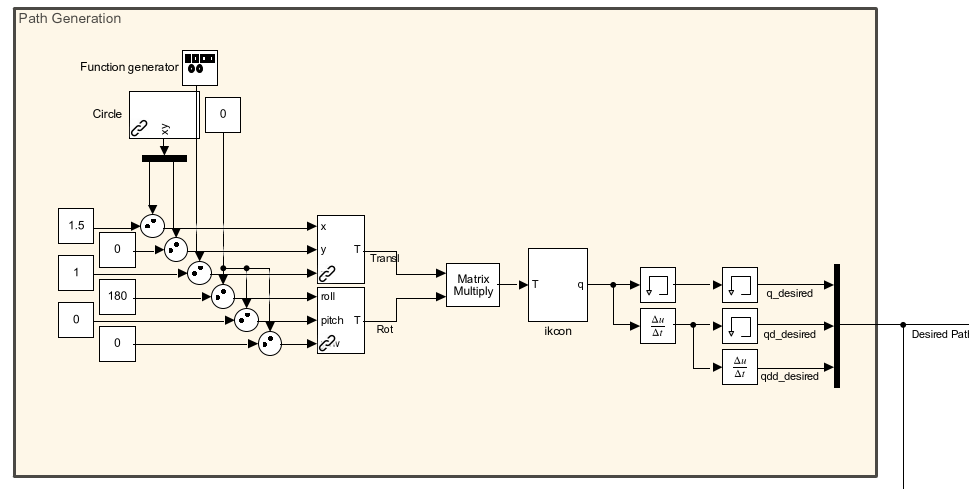
\includegraphics[
	width=1\linewidth,
	center,
	keepaspectratio,
	]{controlScheme/ComputedTorqueControl_Simulink_Input}
	\caption{Path Generation in Simulink for Computed Torque Control}
	\label{fig:PathGen}
\end{figure}

The path generation for workspace control is similar. Here, no inverse kinematics is needed as the desired Transformation matrix can be directly handed to the controller. 

\section{Performance of the control}

With the model and control implemented in MATLAB, the performance of the control schemes can be analysed.
The performance of the two control strategies can be observed with different inputs.
Following inputs are tested:
\begin{itemize}
	\item Point to Point
	\item 3D-Path tracking
\end{itemize}
For the point to point motion, the robot is initialized in normal pose. Then, a desired position with zero offset in Z and a change in X and Y-position compared to normal pose is given to the controller.
The 3D-Path tracking is observed on a circular path in the X/Y plane with a sinusoid on the Z-axis.


\subsection{Computed Torque Control}

\paragraph{Point to Point}
The Path in the X/Y plane can be seen in figure  \ref{fig:XYPPCompTorq}. 
%plot(Rsim.X.Data,Rsim.Y.Data) 
It can be clearly seen, that the robot takes a curved path to the desired end position, as the shortest path in joint space is taken.
\begin{figure}[H]
	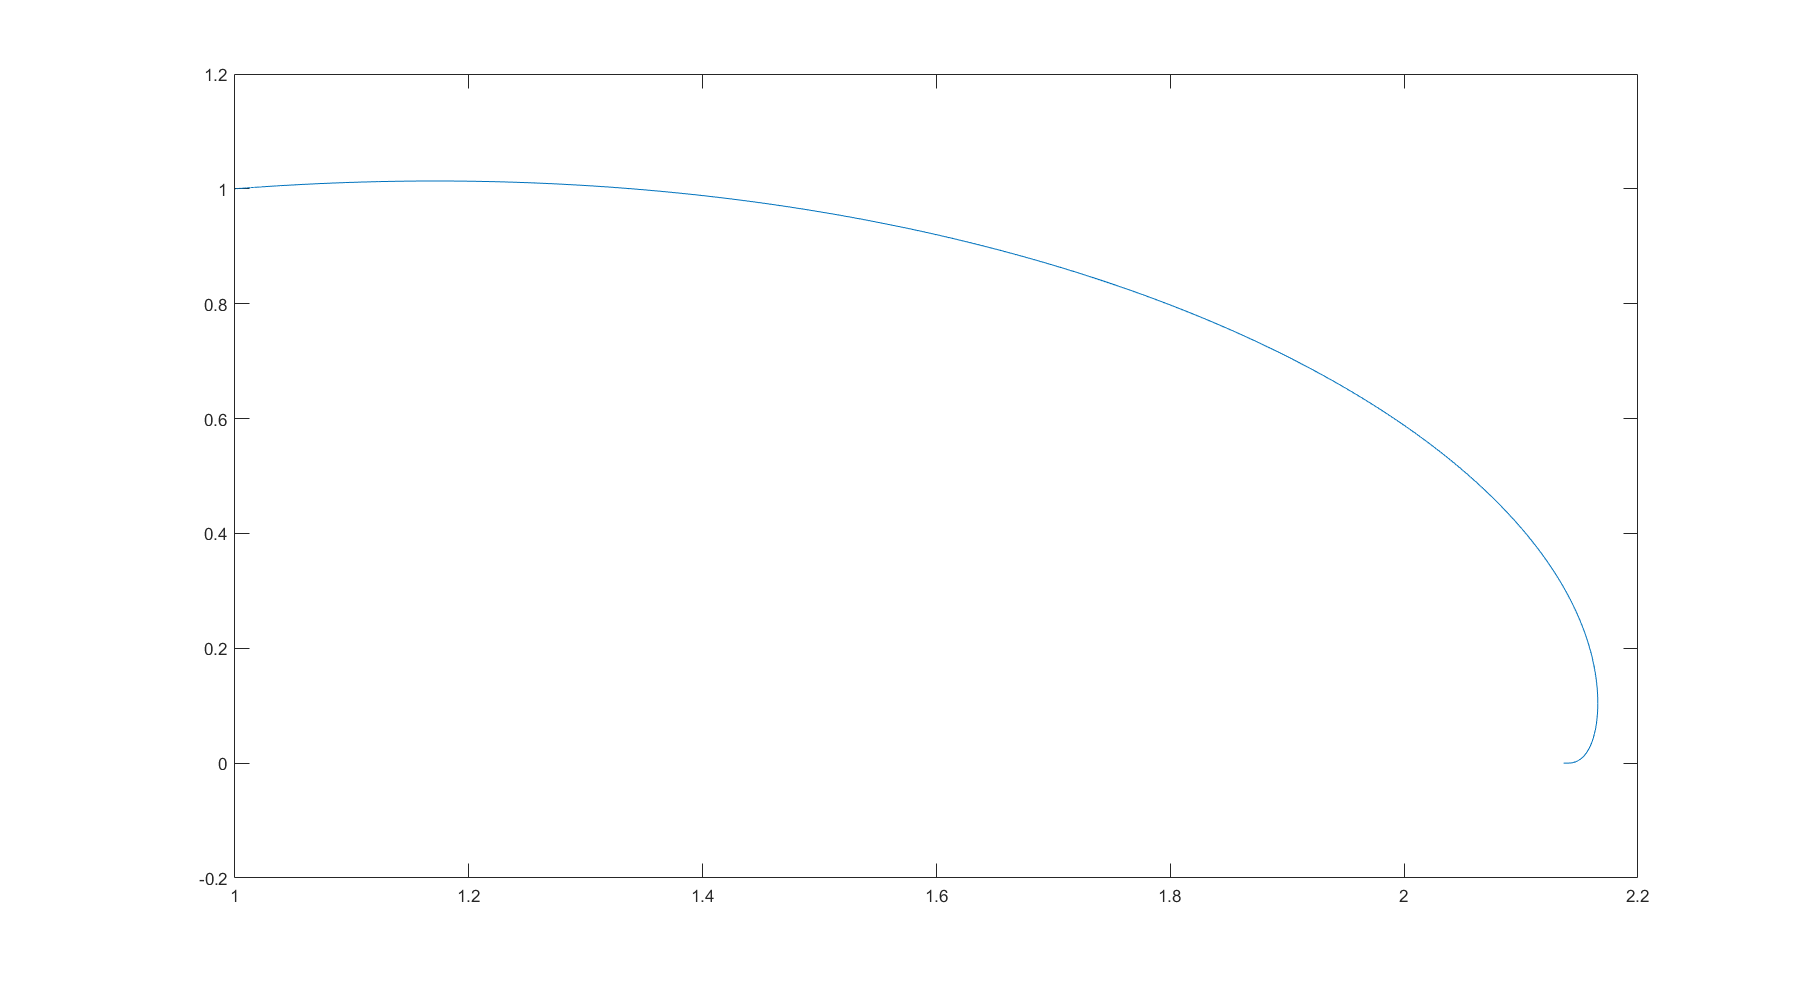
\includegraphics[
	width=1\linewidth,
	center,
	keepaspectratio,
	]{Results/XYPPCompTorq}
	\caption{Path in X/Y plane for point to point motion with computed torque control}
	\label{fig:XYPPCompTorq}
\end{figure}
The errors in XYZ-position can be seen in figure \ref{fig:XYZerrPPCompTorq}. %plot(Rsim.X_err.Time,Rsim.X_err.Data,Rsim.Y_err.Time,Rsim.Y_err.Data,Rsim.Z_err.Time,Rsim.Z_err.Data)
The endeffector reaches its destination straight with no overshoot. It shall be noted here, that the PD-tuning was chosen very low to avoid any overshoot and instabilities. The errors go below 1mm between 3.7 and 5.1 seconds.
\begin{figure}[H]
	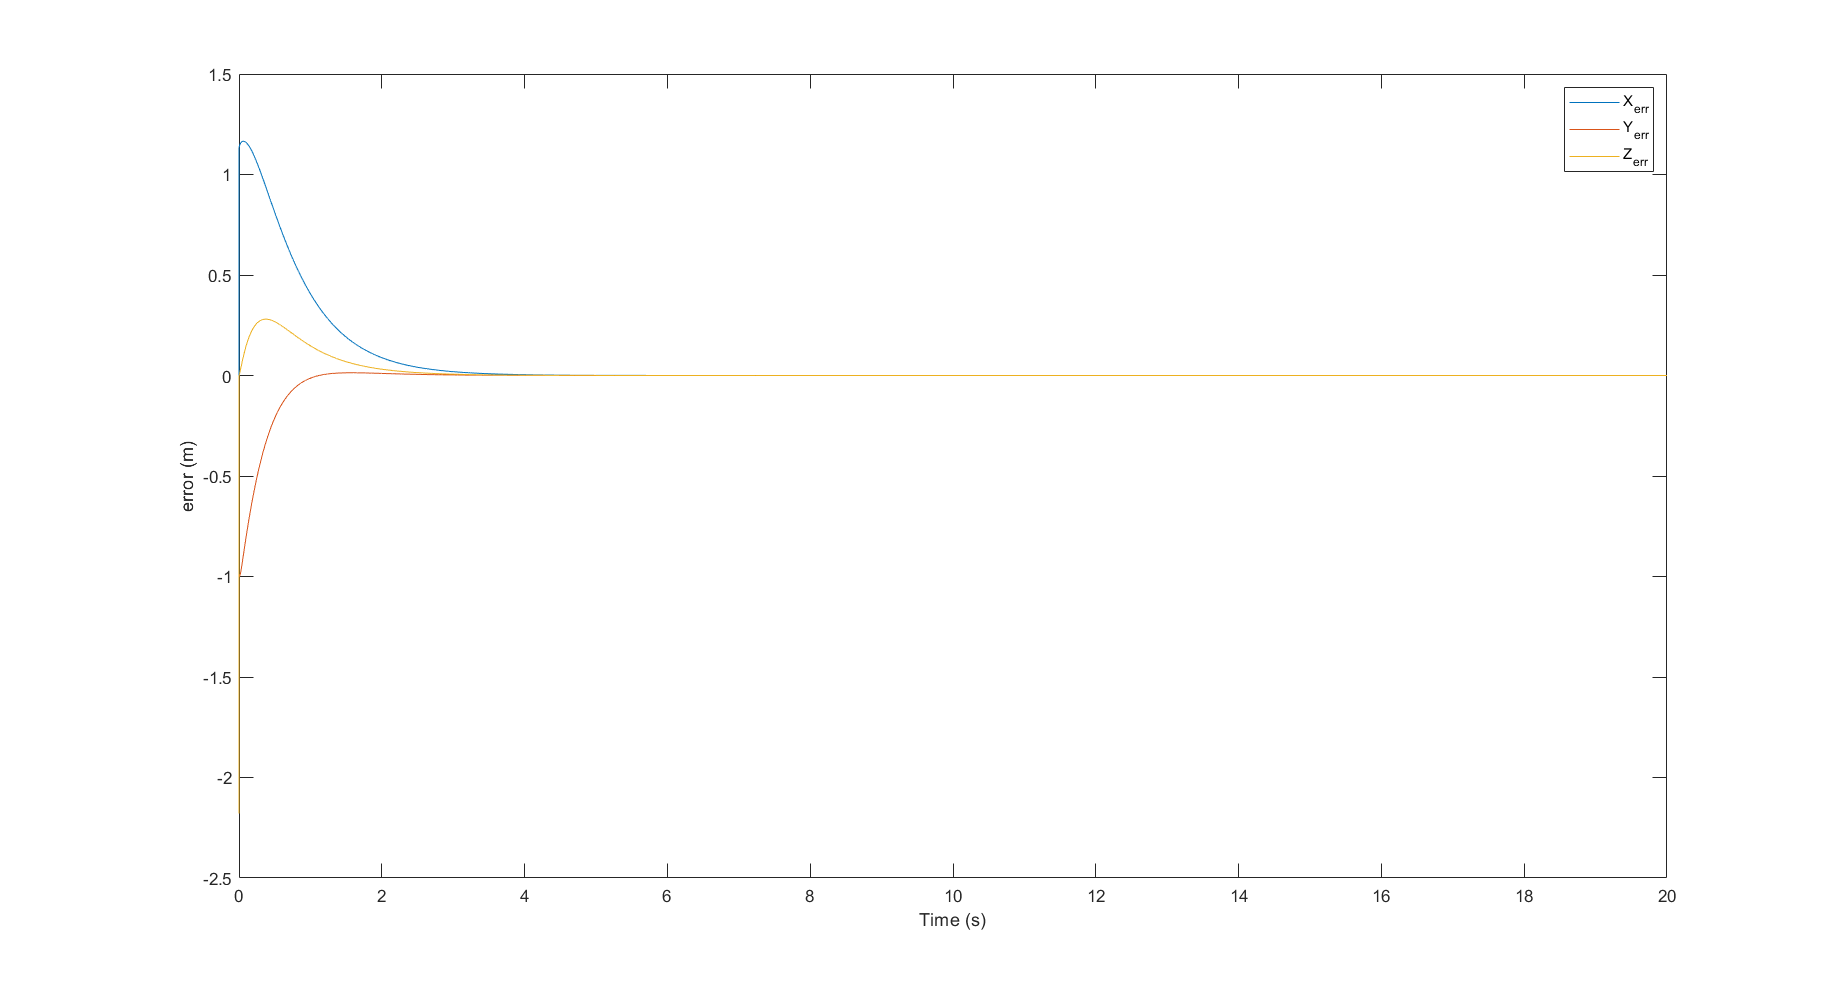
\includegraphics[
	width=1\linewidth,
	center,
	keepaspectratio,
	]{Results/XYZerrPPCompTorq}
	\caption{Errors in XYZ-position for point to point motion with computed torque control}
	\label{fig:XYZerrPPCompTorq}
\end{figure}


%\begin{figure}[H]
%	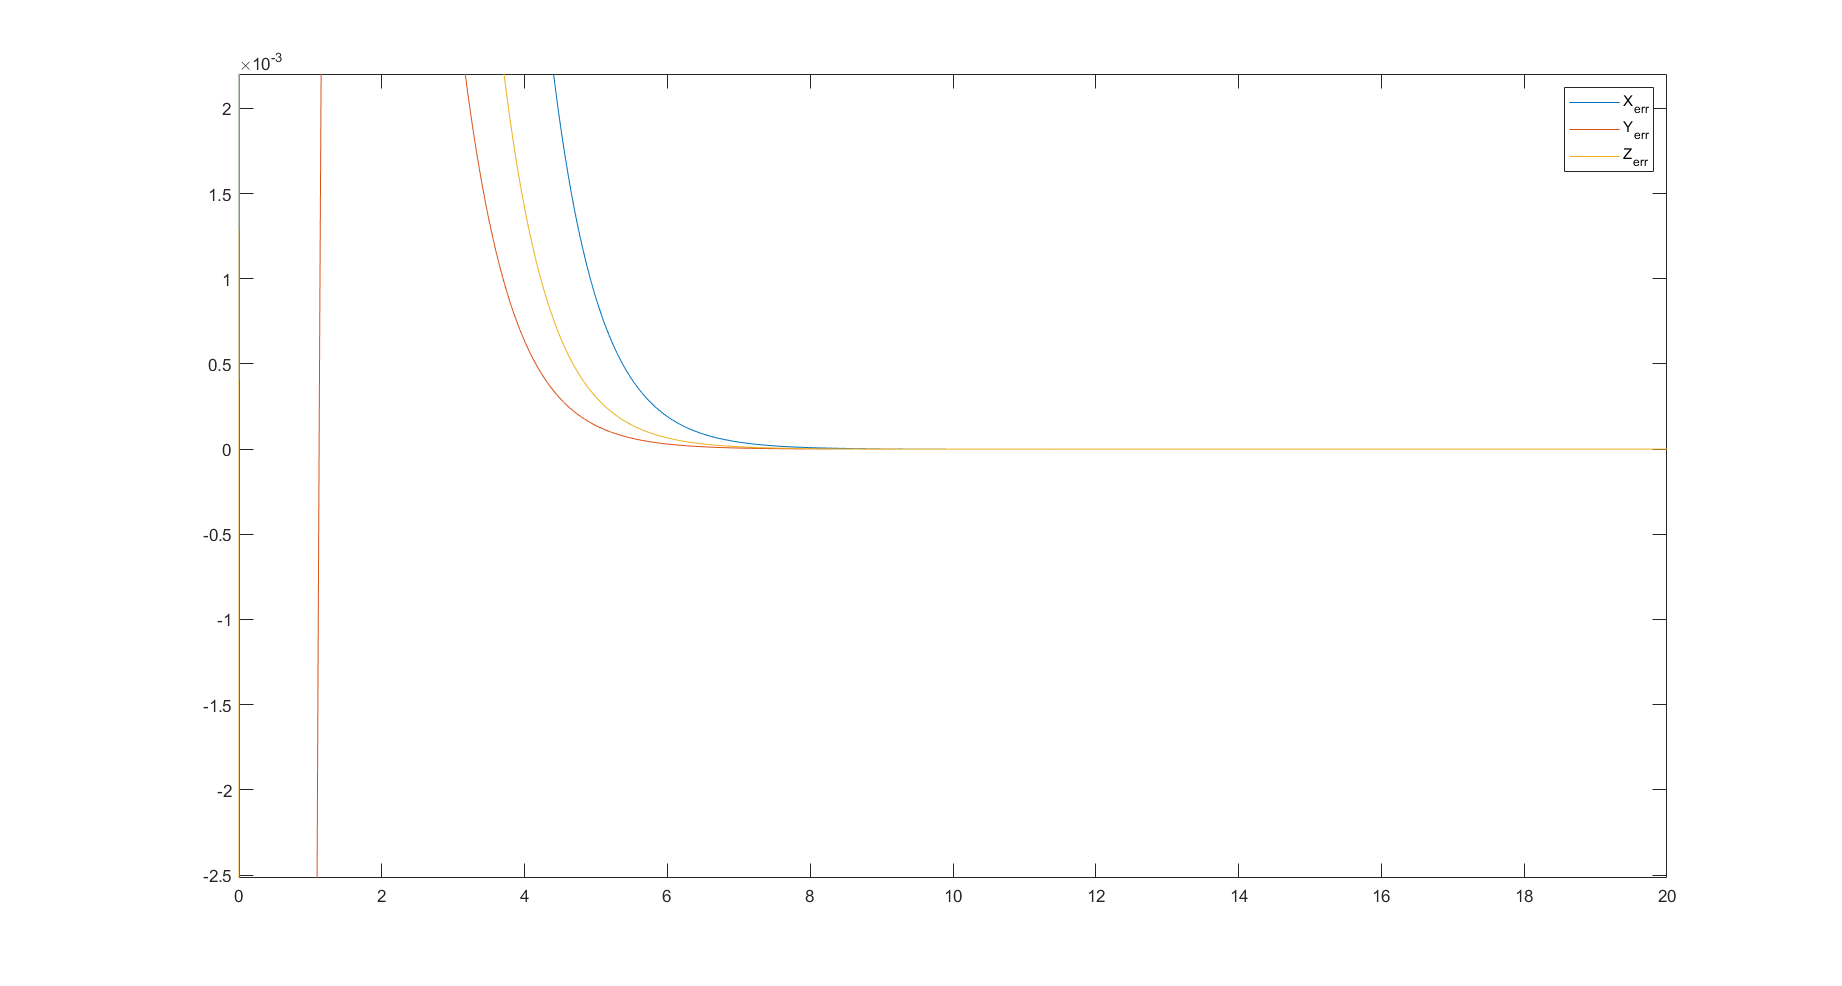
\includegraphics[
%	width=1\linewidth,
%	center,
%	keepaspectratio,
%	]{Results/XYZerrPPCompTorq_zoom3}
%	\caption{Errors in XYZ-position for point to point motion with computed torque control zoomed in}
%	\label{fig:XYZerrPPCompTorq}
%\end{figure}

\paragraph{3D-Path}

The XYZ position vs the desired XYZ path can be seen in figure \ref{fig:XYZposVsdesPosCompTorq}% plot(Rsim.X.Time,Rsim.X.Data,Rsim.Y.Time,Rsim.Y.Data,Rsim.Z.Time,Rsim.Z.Data,Rsim.X_des.Time,Rsim.X_des.Data,Rsim.Y_des.Time,Rsim.Y_des.Data,Rsim.Z_des.Time,Rsim.Z_des.Data)
% legend('X','Y','Z','X_{des}','Y_{des}','Z_{des}')
After a short Synchronization time due to difference in initial position, the end effector follows the desired trajectory.
\begin{figure}[H]
	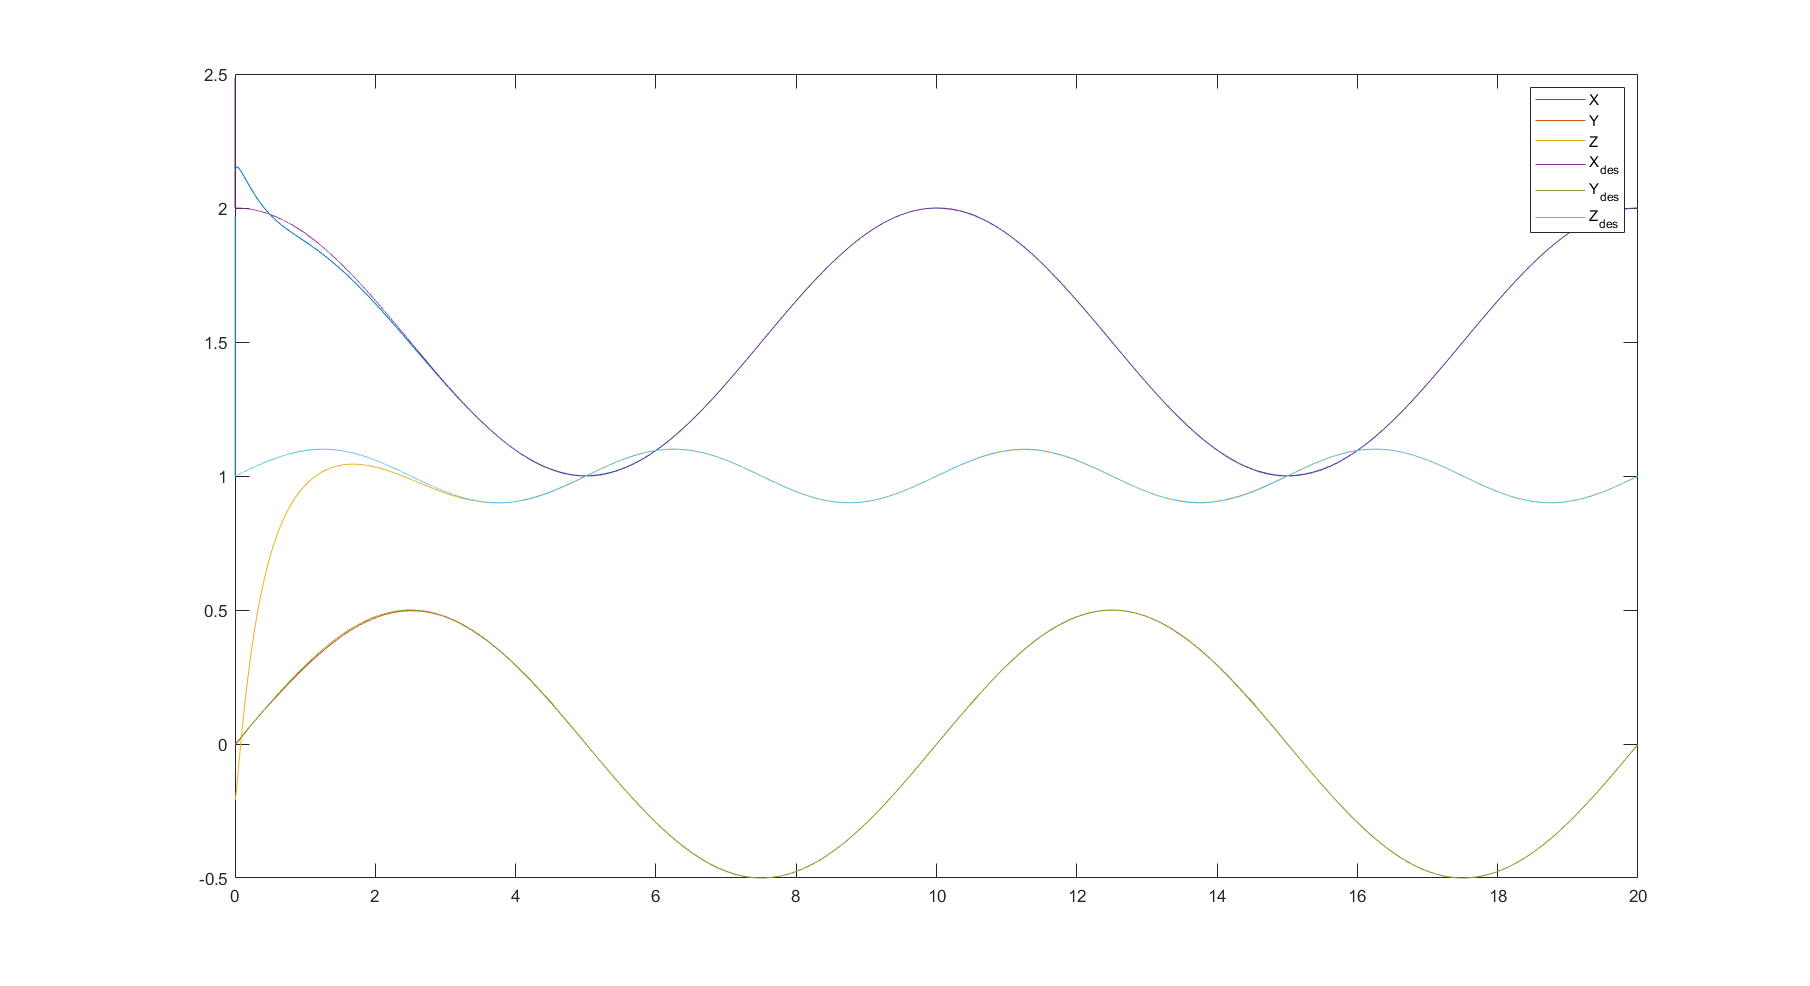
\includegraphics[
	width=1\linewidth,
	center,
	keepaspectratio,
	]{Results/XYZposVsdesPosCompTorq}
	\caption{XYZ-position vs desired XYZ path with computed torque control}
	\label{fig:XYZposVsdesPosCompTorq}
\end{figure}
The errors in XYZ-tracking can be seen in figure \ref{fig:XYZerrPathCompTorq} %plot(Rsim.X_err.Time,Rsim.X_err.Data,Rsim.Y_err.Time,Rsim.Y_err.Data,Rsim.Z_err.Time,Rsim.Z_err.Data)
%legend('X_{err}','Y_{err}','Z_{err}')
For the trajectory tracking, an overshoot in x-direction can be observed, that settles with the error in z-direction. 
Even after the synchronization period, very small tracking errors appear. These are results of the coupled non-linearities.
\begin{figure}[H]
	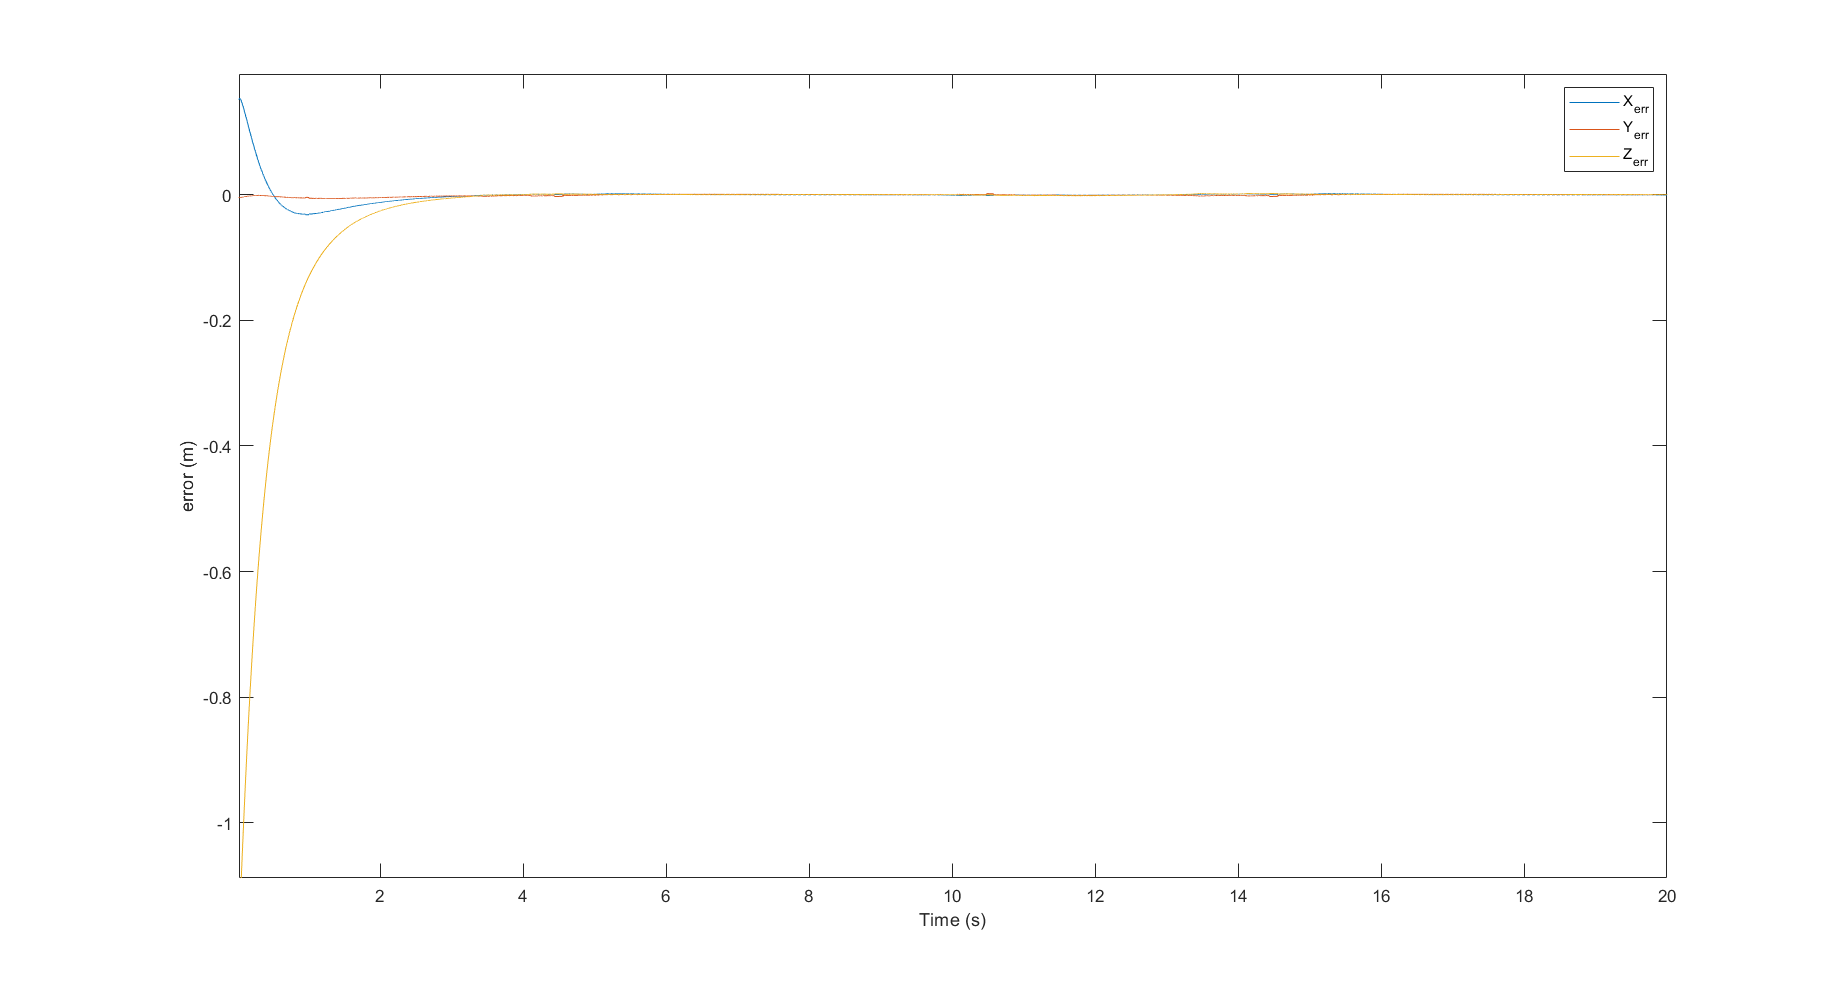
\includegraphics[
	width=1\linewidth,
	center,
	keepaspectratio,
	]{Results/XYZerrPathCompTorq}
	\caption{Errors in XYZ-position for 3D path tracking with computed torque control}
	\label{fig:XYZerrPathCompTorq}
\end{figure}

These overshoots do not occur in the joint space as seen in figure \ref{fig:qerrPathCompTorq}.
\begin{figure}[H]
	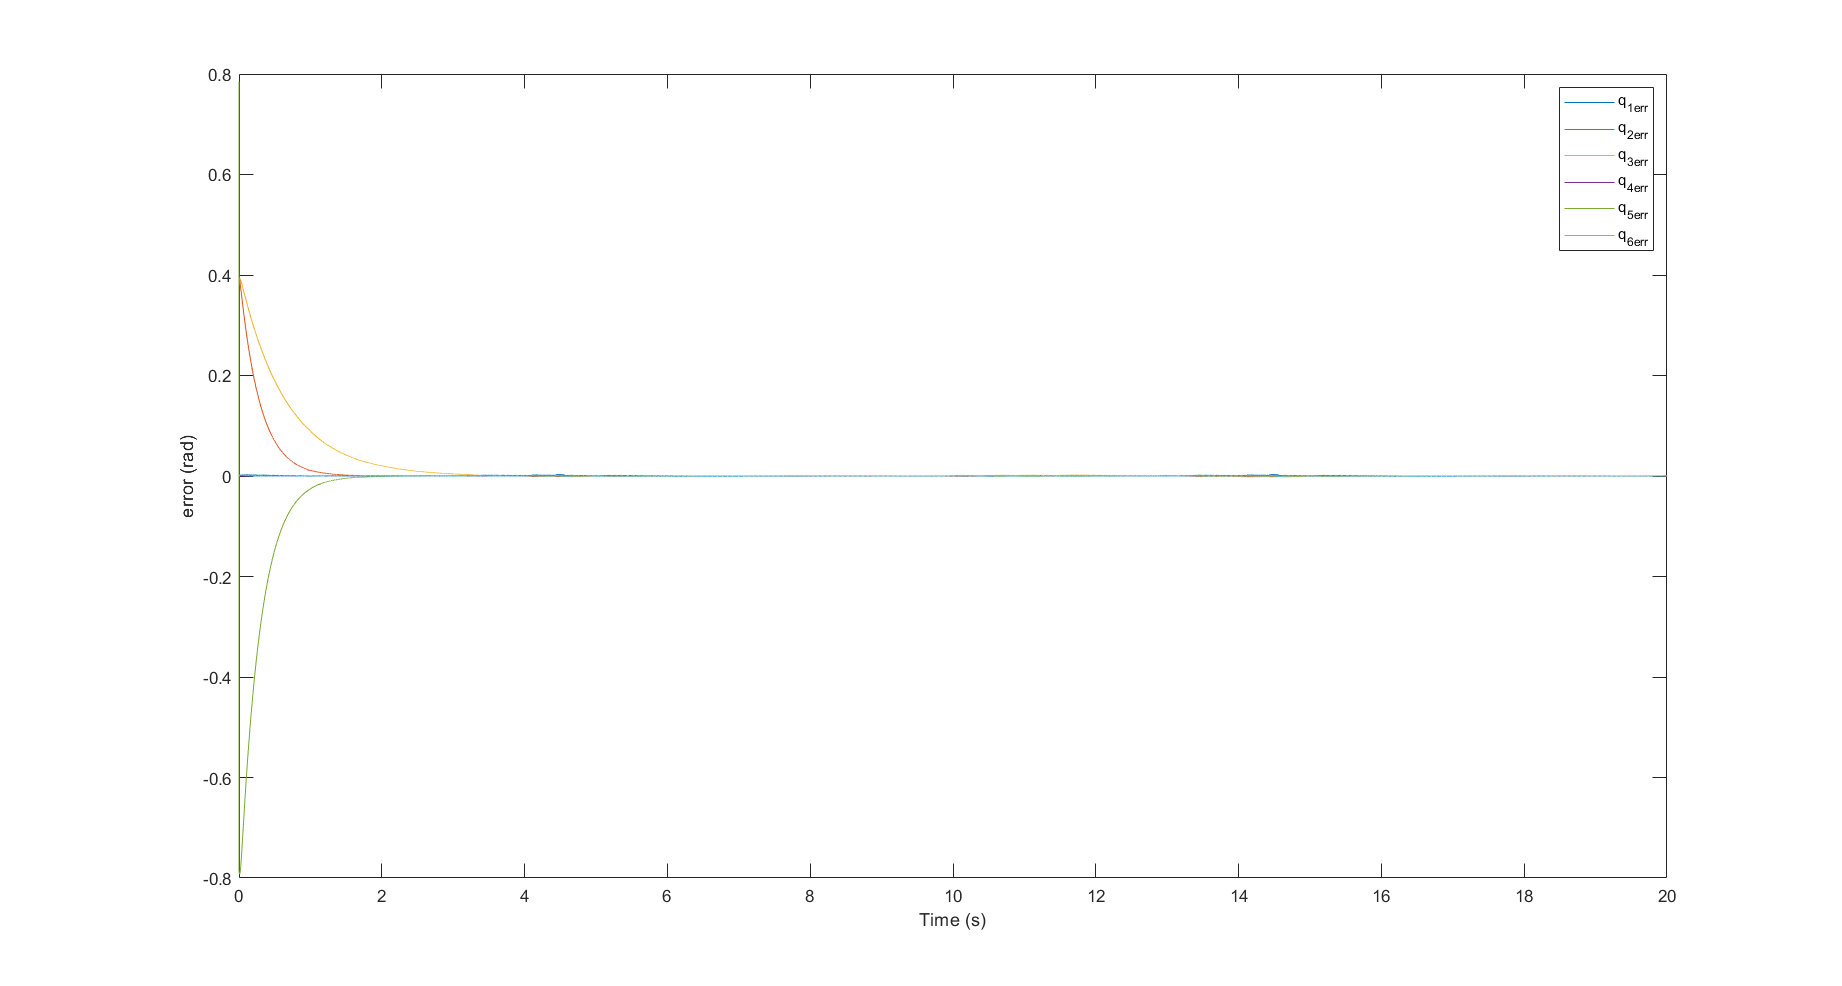
\includegraphics[
	width=1\linewidth,
	center,
	keepaspectratio,
	]{Results/qerrPathCompTorq}
	\caption{Errors in joint space for 3D path tracking with computed torque control}
	\label{fig:qerrPathCompTorq}
\end{figure}




\subsection{Workspace Control}

\paragraph{Point to Point}
The Path in the X/Y plane can be seen in figure  \ref{fig:XYPPWorkspContr}. 
Besides a small movement to the side in the beginning due to the difference in initial conditions, the endeffector follows a straight path to the desired position.
\begin{figure}[H]
	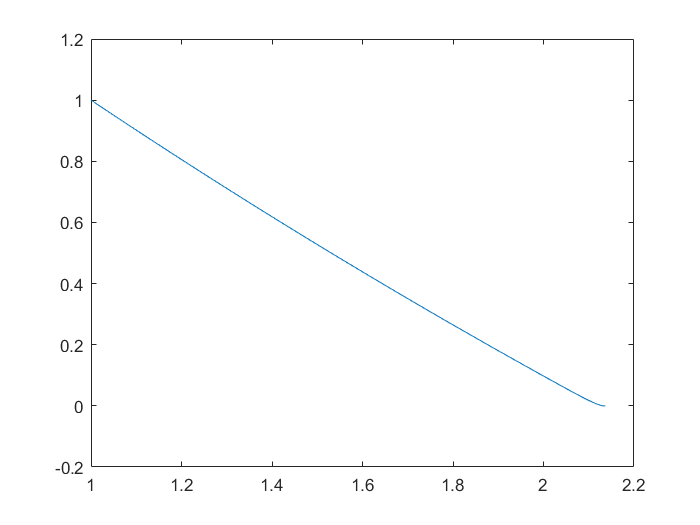
\includegraphics[
	width=1\linewidth,
	center,
	keepaspectratio,
	]{Results/XYPPWorkspContr}
	\caption{Path in X/Y plane for point to point motion with Workspace control}
	\label{fig:XYPPWorkspContr}
\end{figure}
The errors in XYZ-position can be seen in figure \ref{fig:XYZerrPPWorkspContr}.
No overshoot occurs. The endeffector moves straight to the target.
\begin{figure}[H]
	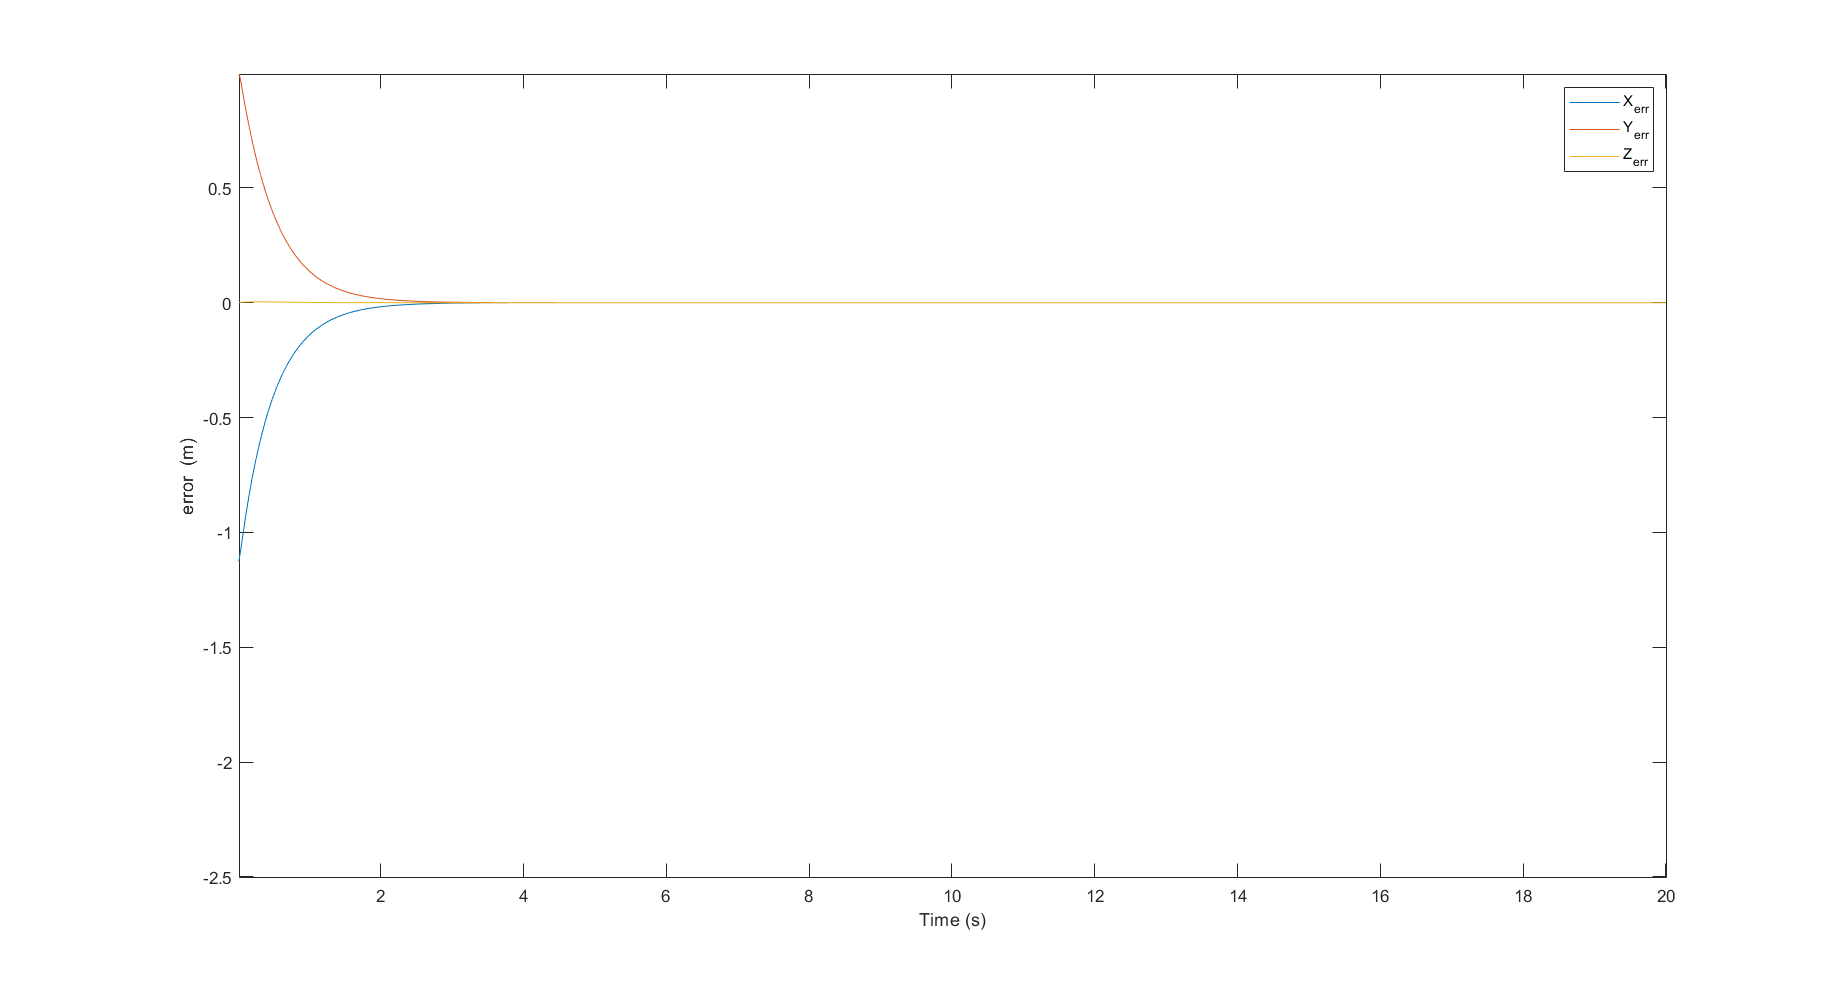
\includegraphics[
	width=1\linewidth,
	center,
	keepaspectratio,
	]{Results/XYZerrPPWorkspContr}
	\caption{Errors in XYZ-position for point to point motion with Workspace control}
	\label{fig:XYZerrPPWorkspContr}
\end{figure}

For point to point tracking, it is advised to turn off the acceleration and velocity feedforward to avoid unreasonable spikes in joint torques.

\paragraph{3D-Path}
The XYZ position vs the desired XYZ path can be seen in figure \ref{fig:XYZposVsdesPosWorkspContr}
After a short Synchronization time due to difference in initial position, the end effector follows the desired trajectory.
\begin{figure}[H]
	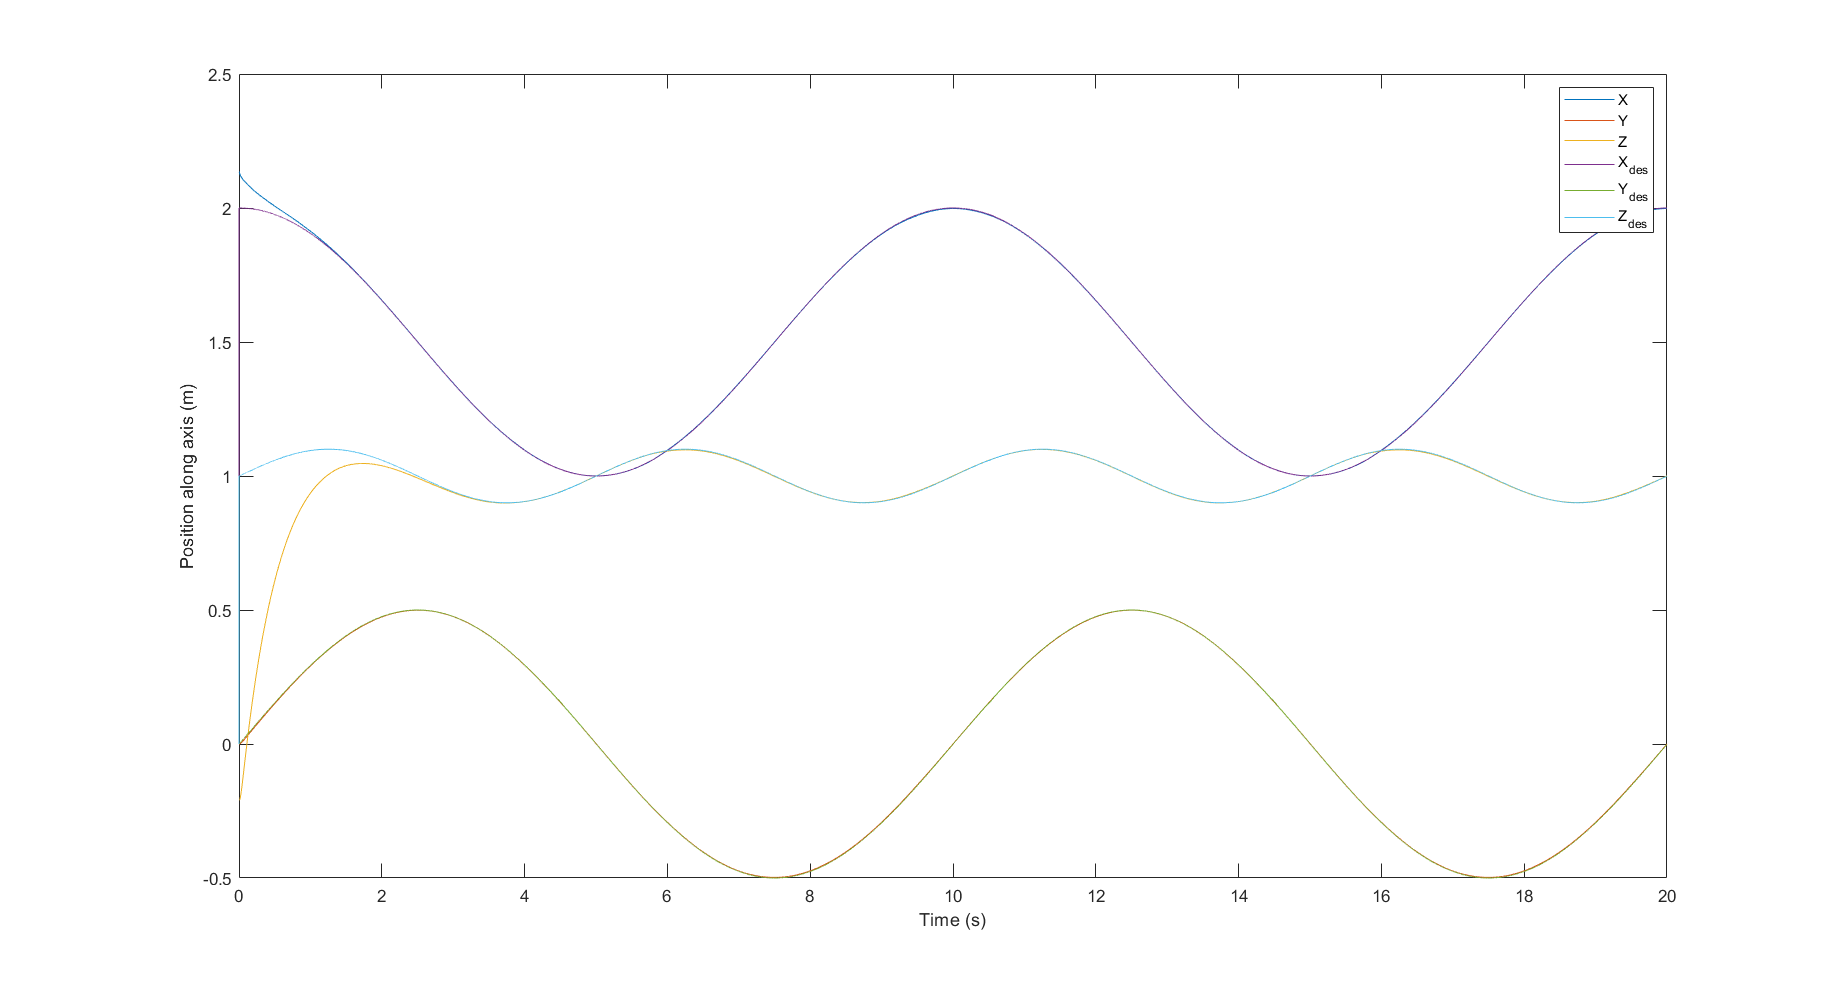
\includegraphics[
	width=1\linewidth,
	center,
	keepaspectratio,
	]{Results/XYZposVsdesPosWorkspContr}
	\caption{XYZ-position vs desired XYZ path with Workspace control}
	\label{fig:XYZposVsdesPosWorkspContr}
\end{figure}
The errors in XYZ-tracking can be seen in figure \ref{fig:XYZerrPathWorkspContr}
No overshoot can be seen. After the synchronization period, small tracking errors that vary with the path appear. These could probably be mitigated with a more aggressive PD tuning.
\begin{figure}[H]
	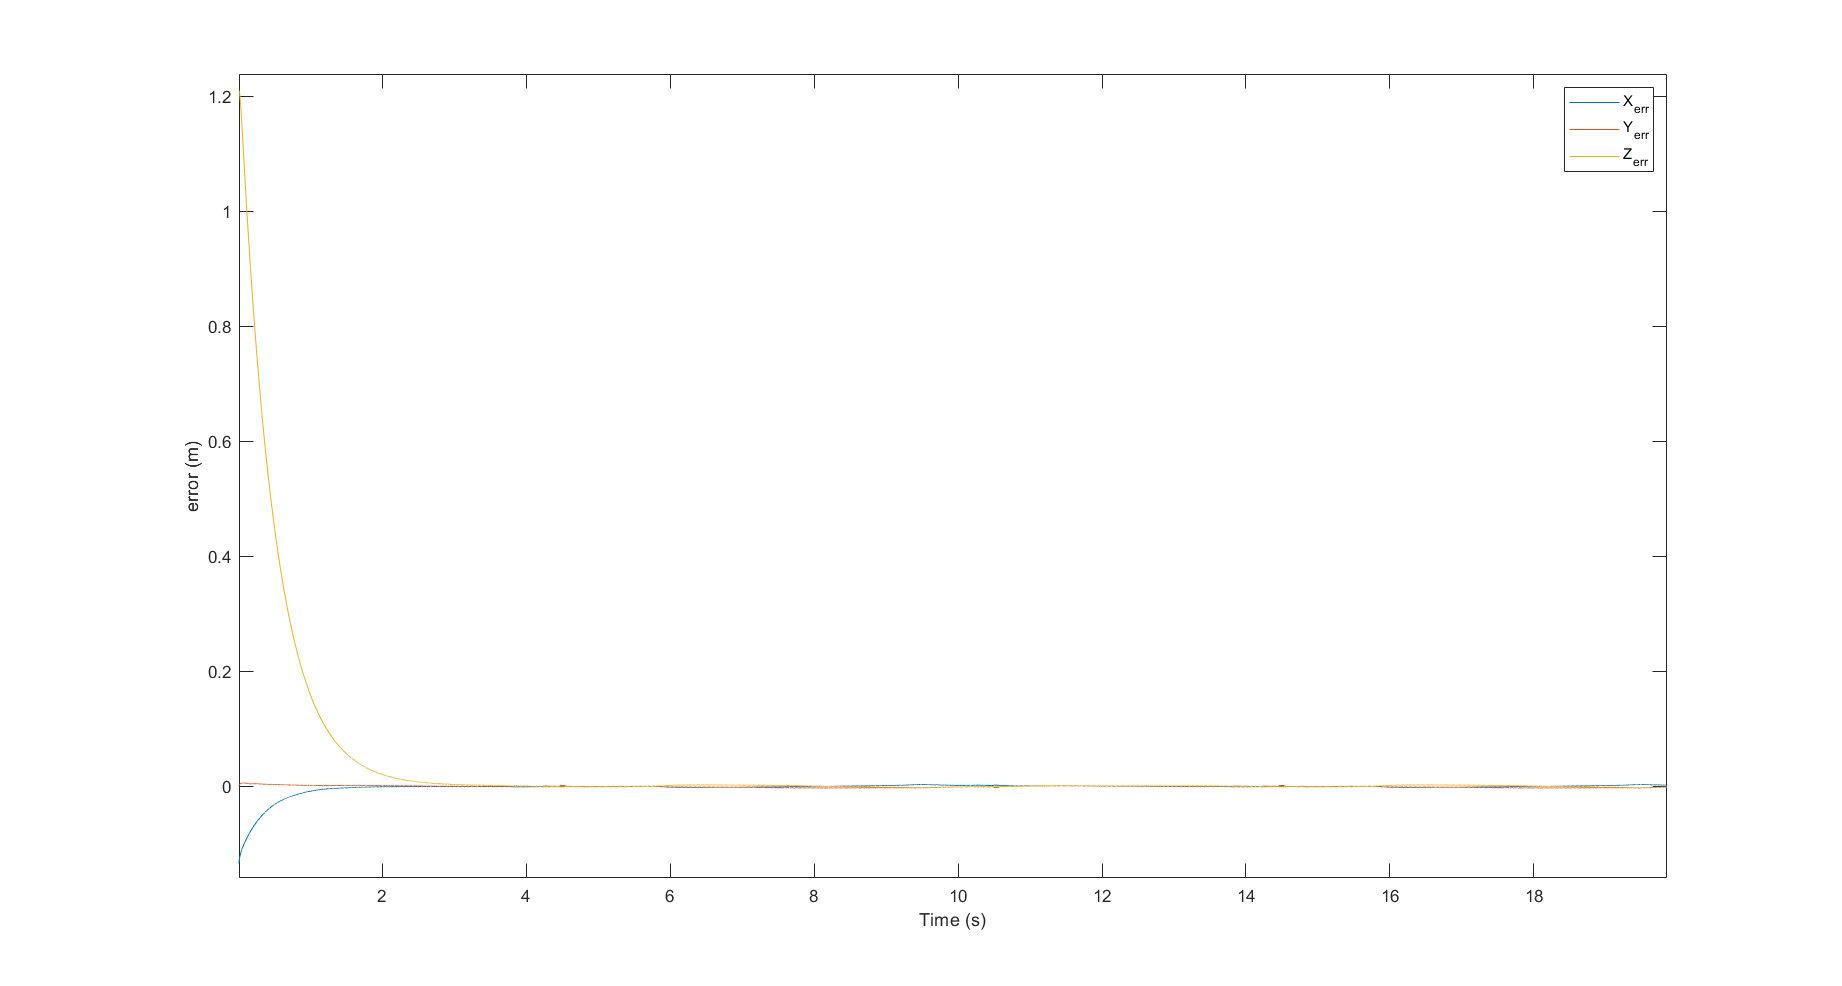
\includegraphics[
	width=1\linewidth,
	center,
	keepaspectratio,
	]{Results/XYZerrPathWorkspContr}
	\caption{Errors in XYZ-position for 3D path tracking with Workspace control}
	\label{fig:XYZerrPathWorkspContr}
\end{figure}


\subsection{Performance comparison of Control strategies}
When comparing figure \ref{fig:XYPPCompTorq} with \ref{fig:XYPPWorkspContr}, it can be seen, that the computed torque control follows a curved line while the workspace control follows a straight line in euclidean space. This is a property of the two control strategies. While the computed torque control follows the shortest distance in joint space, the Workspace control follows the shortest distance in Euclidean space.\\
\\
For point to point motion even with lower PD tuning factors, the Workspace control outperforms the joint space control. as seen in figure \ref{fig:XYZerrPPCompTorqVsWorkspContr}. The error in X-direction settles faster with workspace control. In Z-direction no visible error occurs with workspace control, while with the control in joint space, an overshoot from zero occurs. Only in Y-direction, the joint space control outperforms workspace control.
\begin{figure}[H]
	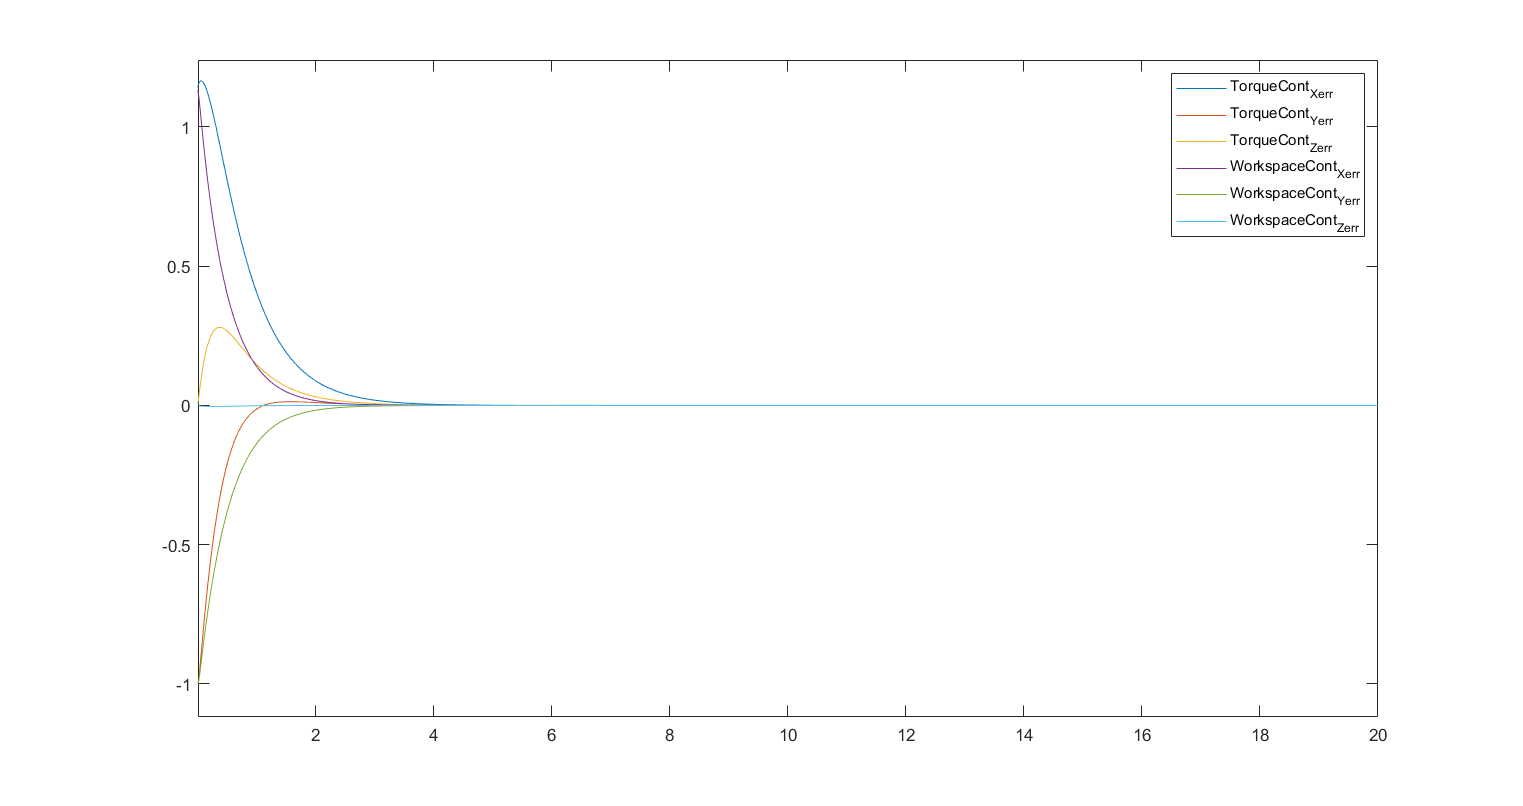
\includegraphics[
	width=1\linewidth,
	center,
	keepaspectratio,
	]{Results/XYZerrPPCompTorqVsWorkspContr}
	\caption{Errors in XYZ-position for 3D path tracking with Computed Torque Control vs Workspace control}
	\label{fig:XYZerrPPCompTorqVsWorkspContr}
\end{figure}

The 3D tracking can be visualized isolated in the XY-plane as seen in figure \ref{fig:XYTrackingPathTorqueContrVsWorkspaceContr}. It can be clearly seen, that the workspace control joins the desired trajectory faster and without overshoot. This is especially of importance when it comes to collision avoidance and applications like \ac{CNC} milling, where overshoot can destroy the product and machine. As the desired path is initialized at zero position in workspace, a jump occurs, that leads to the yellow line in the middle.

\begin{figure}[H]
	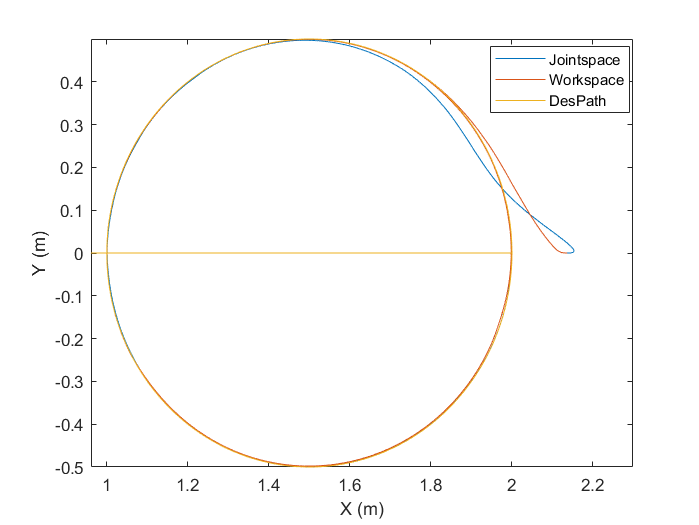
\includegraphics[
	width=1\linewidth,
	center,
	keepaspectratio,
	]{Results/XYTrackingPathTorqueContrVsWorkspaceContr}
	\caption{XY Path Joint Space control vs Workspace Control}
	\label{fig:XYTrackingPathTorqueContrVsWorkspaceContr}
\end{figure}



Overall, the workspace control gives better performance. Also the computational performance is a lot better, as the inverse kinematic problem does not need to be solved.

%It has to be noted though, that the performance in $[Roll,Pitch,Yaw]$ tracking has not been tested, as this would require a

\section{Pick and Place}
The goal of this thesis work is to develop a control strategy for the pick and place operation requested by SPC. A program that can be given to the robot controller can be found in appendix \fullref{TPprogram210F}.
This program defines a sequence of positions. The robot follows these positions to achieve the desired pick and place operation.
The $ [XYZ] $ coordinates can be extracted from this program and fed into the Workspace control simulation.

\subsection{Input sequence}
In figure \ref{fig:PickAndPlace_XYZvsDesXYZ} the desired sequence of positions can be seen, plotted over time. The sequence ends at second $32$ and repeats after that. The positions are given to the controller in an interval of 2 seconds.

\begin{figure}[H]
	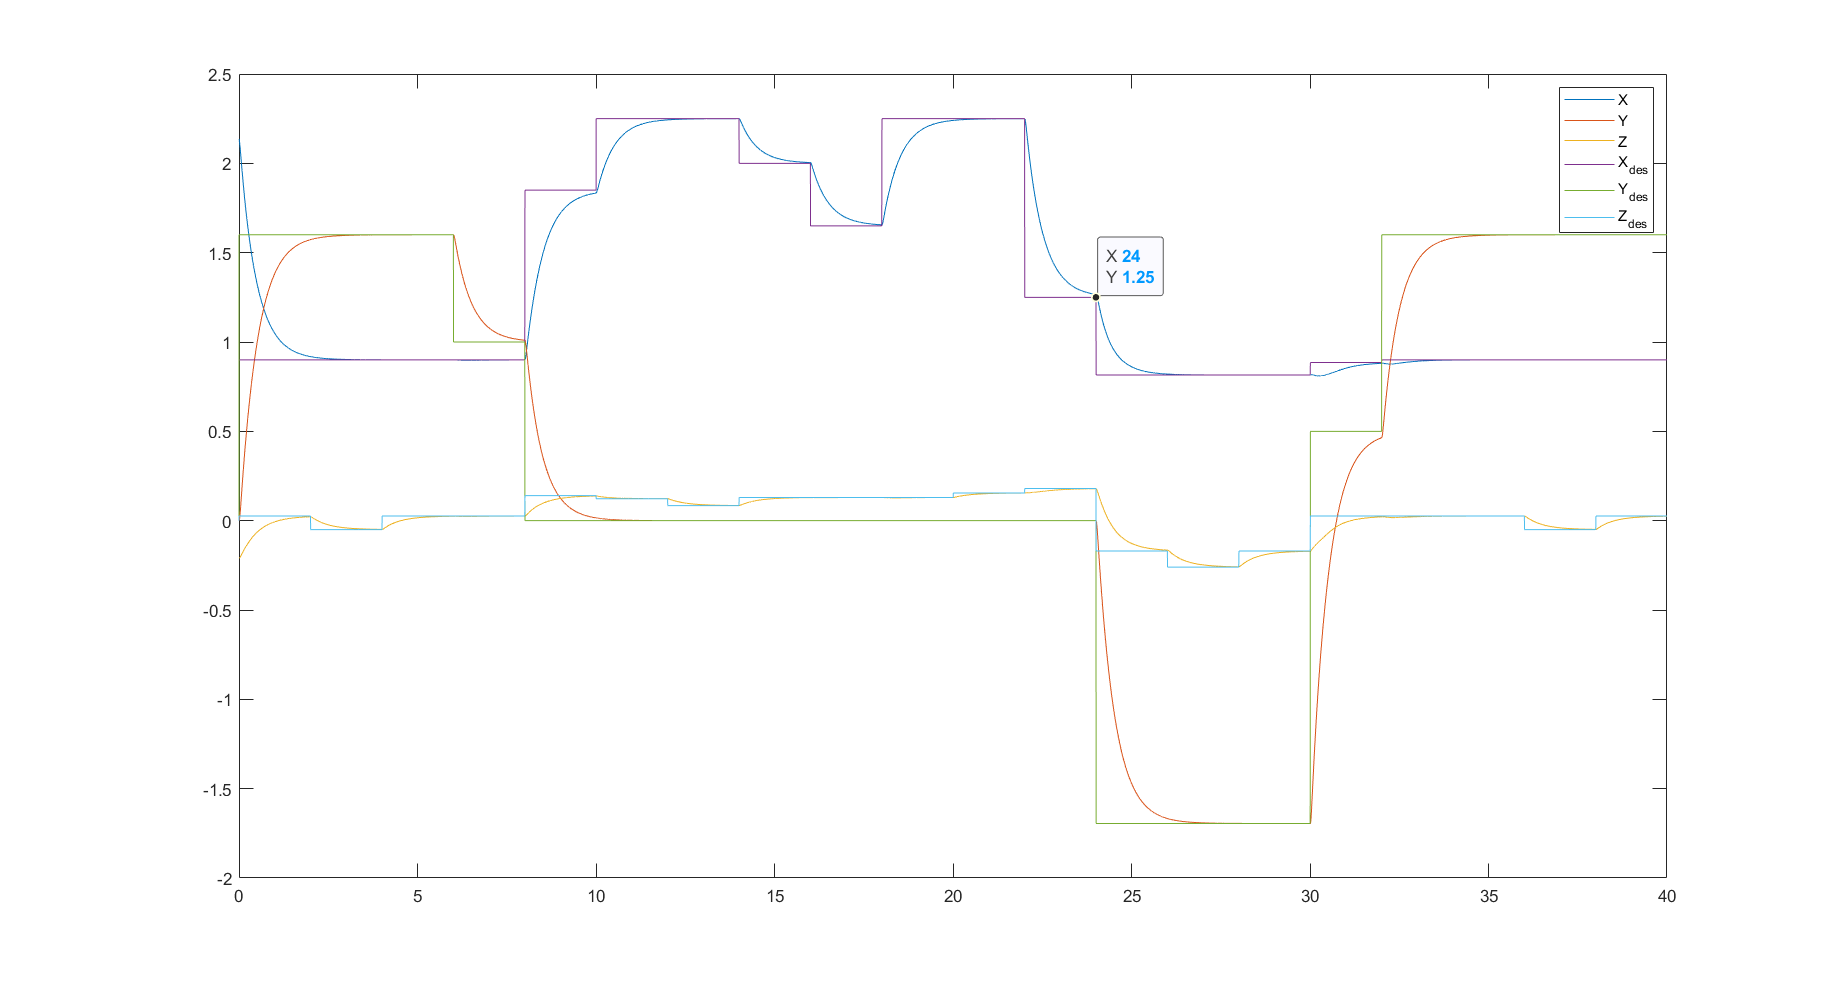
\includegraphics[
	width=1\linewidth,
	center,
	keepaspectratio,
	]{Results/PickAndPlace_XYZvsDesXYZ}
	\caption{XYZ-position vs desired position sequence for pick and place with Workspace control}
	\label{fig:PickAndPlace_XYZvsDesXYZ}
\end{figure}


\subsection{Point Tracking}
As seen in \cref{fig:PickAndPlace_XYZvsDesXYZ} the controller manages to follow the desired sequence of points with some difficulties. Certain points cannot be reached within a 2 second interval time. An example for this tracking error can be seen at second $24$ . In \cref{fig:PickAndPlace_err} an error in x-direction of $0.01605$ can be seen at that point. 
This shows, that not all positions within the workspace of the robot can be reached in 2 seconds with the chosen PD tuning.
Either the tuning needs to be adjusted, or the interval time needs to be increased.

\begin{figure}[H]
	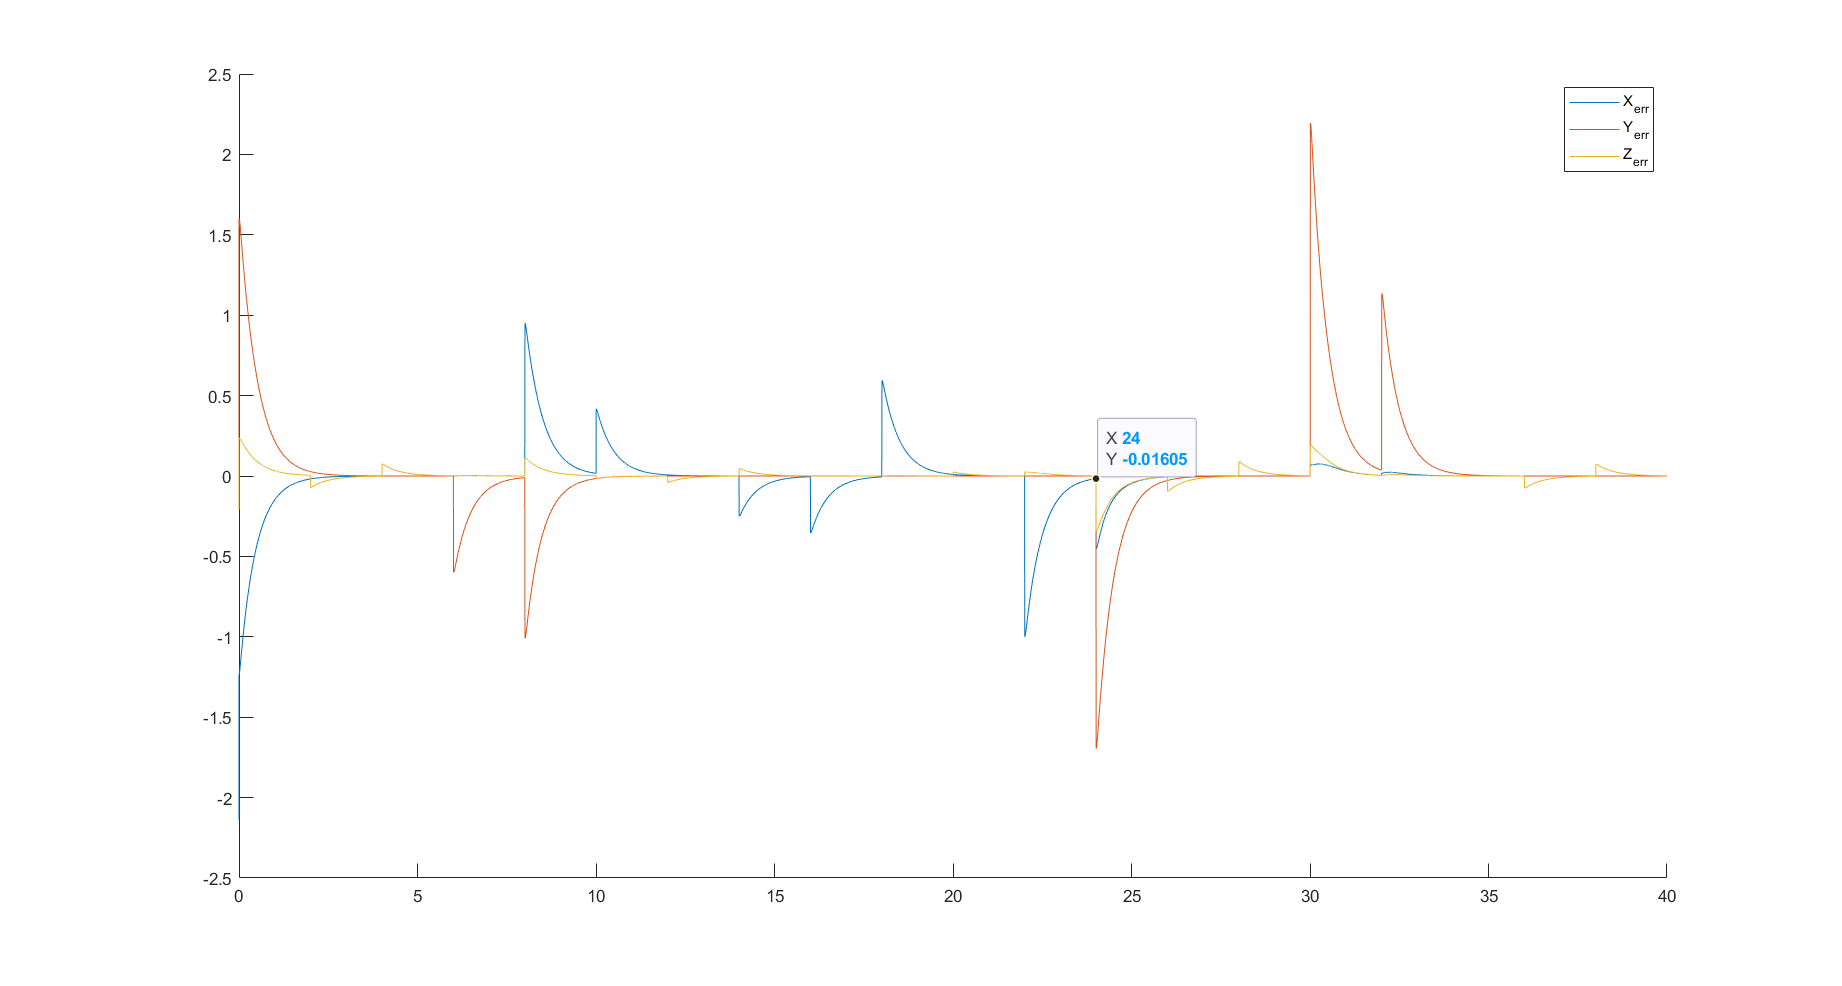
\includegraphics[
	width=1\linewidth,
	center,
	keepaspectratio,
	]{Results/PickAndPlace_err}
	\caption{Errors in XYZ-position for pick and place with Workspace control}
	\label{fig:PickAndPlace_err}
\end{figure}



\subsection{Improvement by Trajectory tracking}
Instead of handing over a set of points to the controller, trajectory tracking can be used to improve the performance for the desired task without making changes to the controller.
For this, interpolated positions are calculated between the desired endpoints.
In \cref{fig:PickAndPlace_InterpTracking_XYZvsDesXYZ} the desired trajectory and the taken path can be seen.
\begin{figure}[H]
	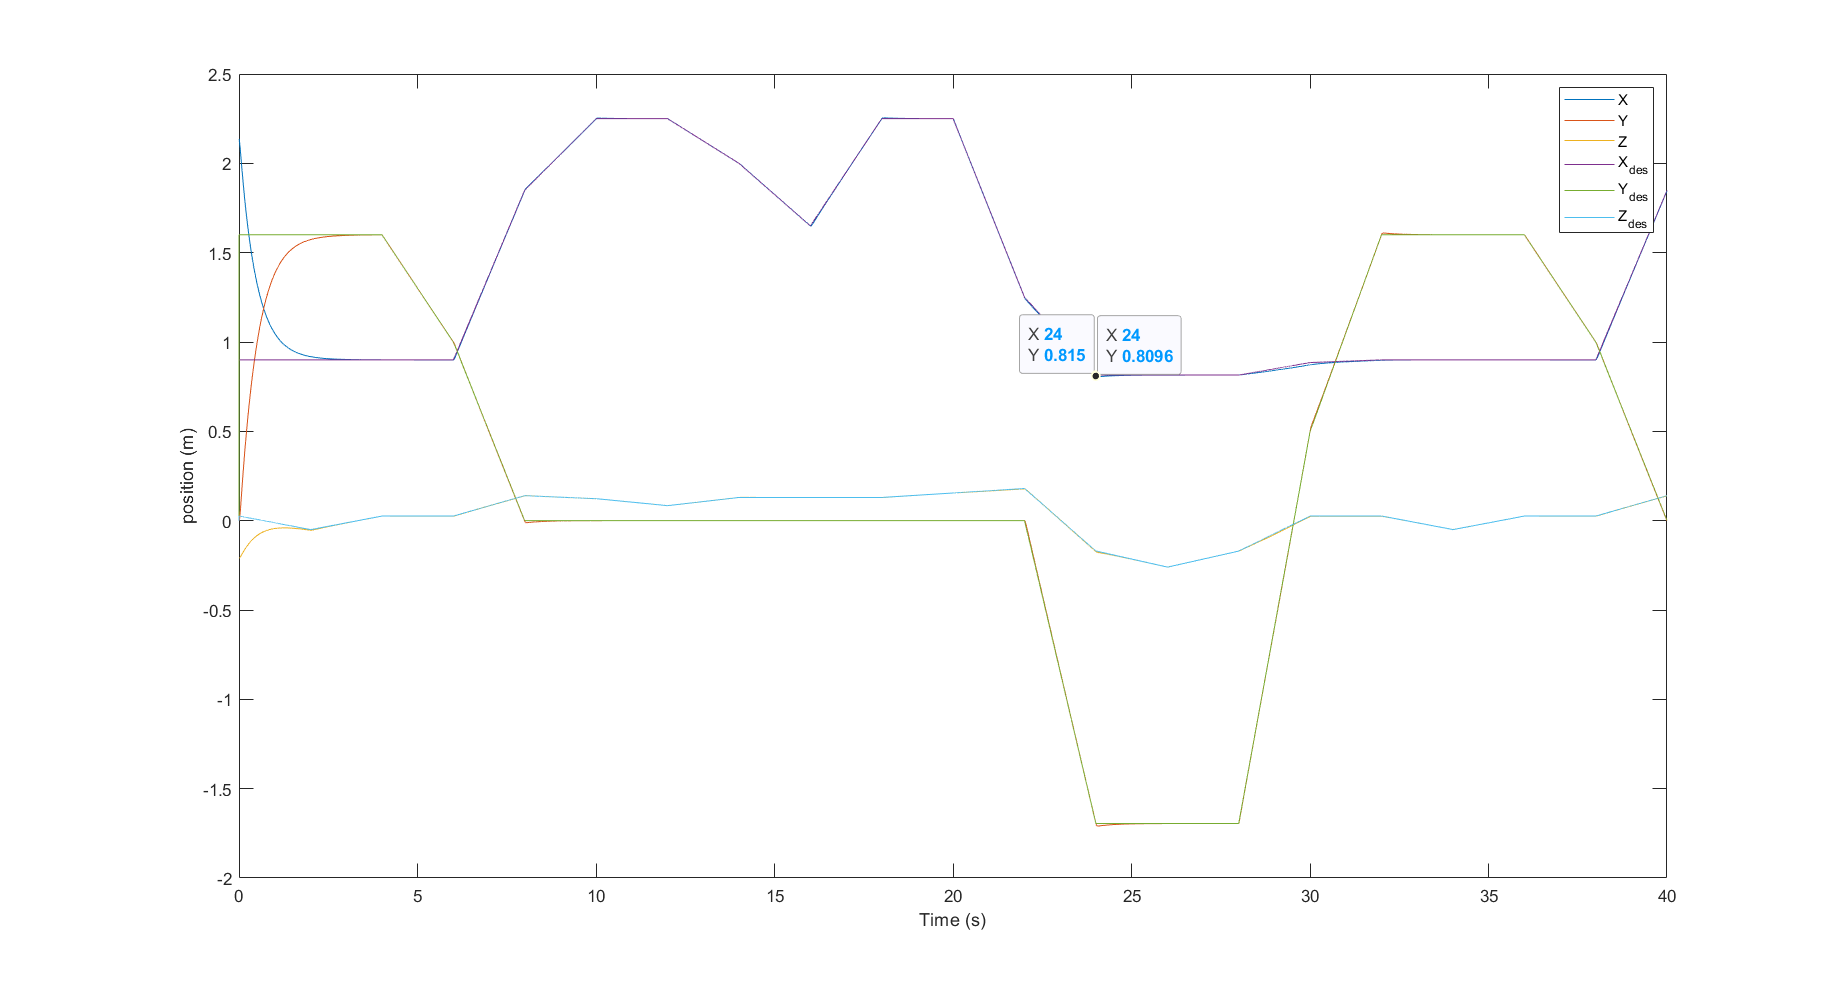
\includegraphics[
	width=1\linewidth,
	center,
	keepaspectratio,
	]{Results/PickAndPlace_InterpTracking_XYZvsDesXYZ}
	\caption{XYZ-position vs desired interpolated path for pick and place with Workspace control}
	\label{fig:PickAndPlace_InterpTracking_XYZvsDesXYZ}
\end{figure}
With this addition, the endeffector manages to reach the desired points within 2 seconds, as velocity and acceleration can be used in the feedforward. The error for the desired position at second $24$ reduces to an overshoot of $0.0054$.

\subsection{Taken path in Workspace}
In \cref{fig:PickAndPlace_XYPlane_WithModel}, the path of the endeffector in the XY plane can be seen with an underlay of the robotic workcell at SPC. The time is represented by colour.
As can be seen, the robot arm travels through itself. This is due to the limitations of this simulation. A collision detection and avoidance is not implemented, as it is computationally expensive. 

\begin{figure}[H]
	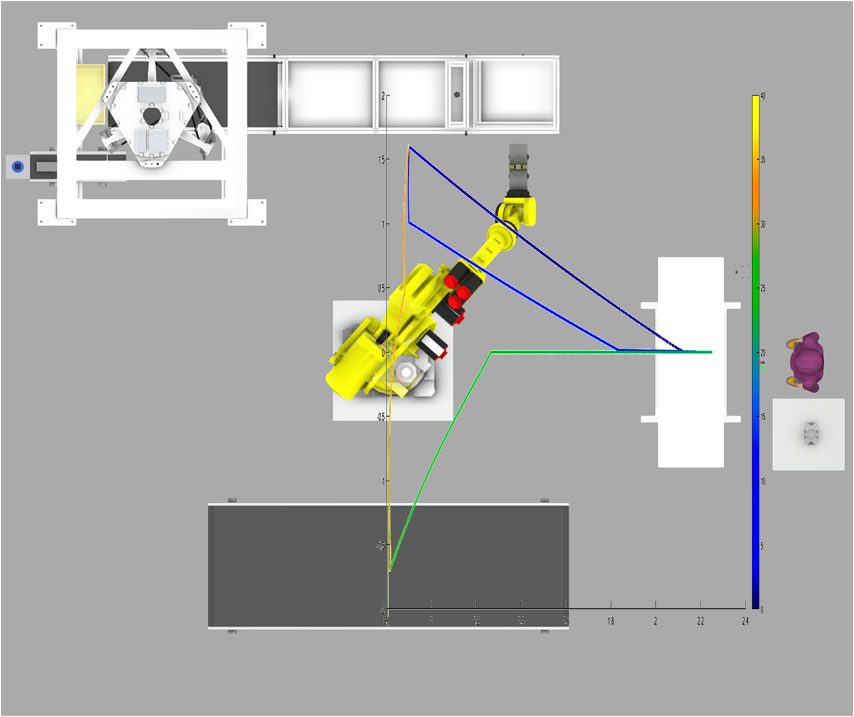
\includegraphics[
	width=1\linewidth,
	center,
	keepaspectratio,
	]{Results/PickAndPlace_XYPlaneTimeColour_transp_WithModel}
	\caption{Path in XY-plane in the robotic work-cell at SPC}
	\label{fig:PickAndPlace_XYPlane_WithModel}
\end{figure}